\begin{figure}[h!]
\centering
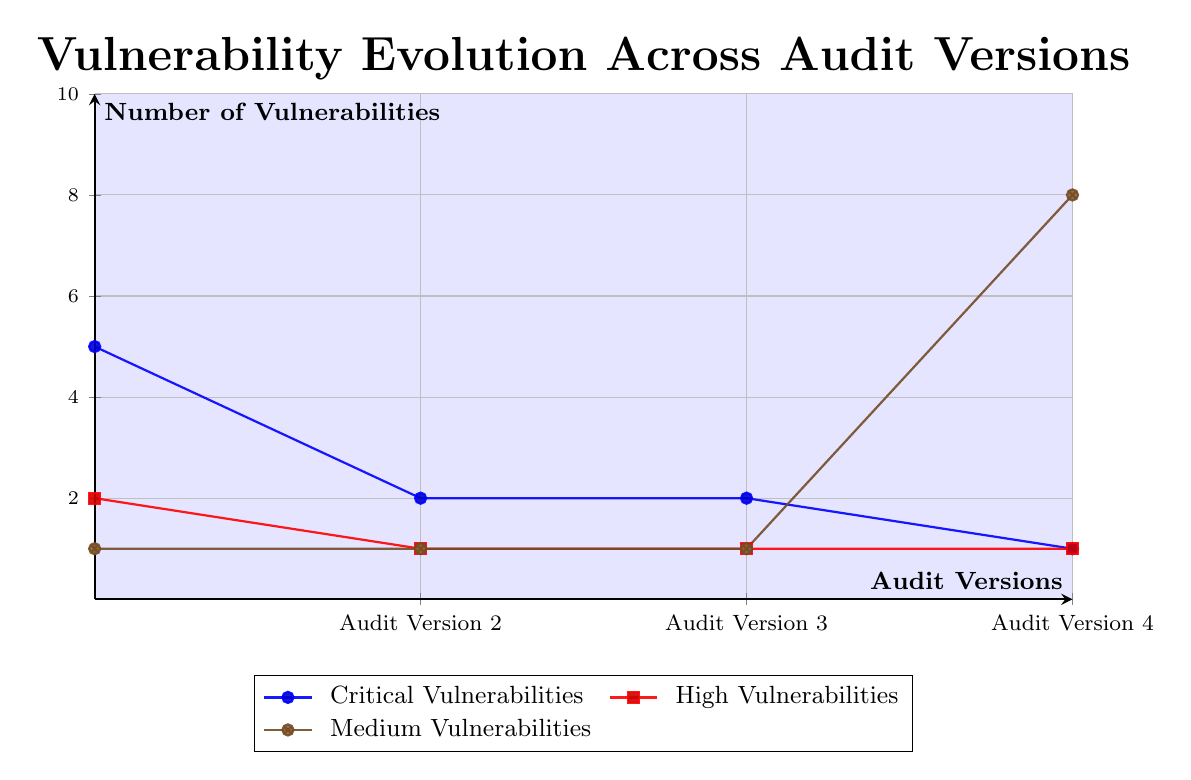
\begin{tikzpicture}
    \begin{axis}[
        axis lines=middle,
        symbolic x coords={Audit Version 1, Audit Version 2, Audit Version 3, Audit Version 4},
        xtick=data,
        ylabel={Number of Vulnerabilities},
        xlabel={Audit Versions},
        ymin=0, ymax=10,
        enlarge x limits=0,
        grid=both,
        title={Vulnerability Evolution Across Audit Versions},
        title style={font=\LARGE\bfseries, color=black, align=center, yshift=-1ex},
        ylabel style={font=\small\bfseries, color=black},
        xlabel style={font=\small\bfseries, color=black},
        tick label style={font=\footnotesize, color=black},
        legend style={
            at={(0.5,-0.15)},
            anchor=north,
            legend columns=2,
            font=\small,
            column sep=1ex,
            text=black,
            legend cell align=left
        },
        width=14cm, height=8cm,
        yticklabel style={font=\scriptsize},
        axis line style={draw=black, thick},
        every axis plot/.append style={thick, mark=none, opacity=0.9, color=red},
        % === NUEVO: Fondo para el gráfico ===
        area background/.style={fill=blue!10},
        axis background/.style={fill=blue!10},
    ]

    % Leyenda
    \legend{Critical Vulnerabilities, High Vulnerabilities, Medium Vulnerabilities}

    % Ejemplo de líneas si querés verlas funcionando:
    \addplot coordinates {(Audit Version 1,5) (Audit Version 2,2) (Audit Version 3,2) (Audit Version 4,1)};
     \addplot coordinates {(Audit Version 1,2) (Audit Version 2,1) (Audit Version 3,1) (Audit Version 4,1)};
    \addplot coordinates {(Audit Version 1,1) (Audit Version 2,1) (Audit Version 3,1) (Audit Version 4,8)};

    \end{axis}
\end{tikzpicture}
\caption{Vulnerability Evolution Across Audit Versions (With Trend Lines)}
\end{figure}
